\documentclass[11pt,a4paper]{article}

\usepackage[margin=2.5cm]{geometry}
\usepackage{amsmath,amssymb}
\usepackage{graphicx}
\usepackage{booktabs}
\usepackage{hyperref}
\usepackage{xcolor}
\usepackage{caption}
\usepackage{subcaption}
\usepackage{float}
\usepackage{microtype}
\usepackage{parskip}

\hypersetup{
  colorlinks=true,
  linkcolor=blue!60!black,
  citecolor=blue!60!black,
  urlcolor=blue!60!black,
}

\title{\textbf{Membership Inference Attacks on a Fine-tuned\\
Masked Diffusion Language Model}\\[0.5em]
\large Run 1 --- Qwen3-0.6B MDLM (DLLM-Hub)}

\author{DA5001 Project\\
Indian Institute of Technology Madras}

\date{April 2026}

\begin{document}

\maketitle
\tableofcontents
\newpage

% ============================================================
\section{Overview}
% ============================================================

This report documents the first full experimental run of a membership inference
attack (MIA) pipeline targeting a masked diffusion language model (MDLM).
The pipeline is composed of seven stages:

\begin{enumerate}
  \item \textbf{Data preparation} --- sample 300 member and 300 non-member texts
        from the MIMIR GitHub benchmark.
  \item \textbf{Fine-tuning} --- overfit the base model on member data to induce
        memorization.
  \item \textbf{Memorization verification} --- confirm that fine-tuning produced a
        measurable ELBO gap before running expensive signal extraction.
  \item \textbf{SAMA baseline} --- run the black-box reference-model attack
        (Algorithm 1+2 from~\cite{sama}).
  \item \textbf{White-box signal extraction} --- compute a 112-dimensional feature
        vector per sample using \texttt{extract\_metrics()}.
  \item \textbf{Classifier training} --- train XGBoost and MLP on the extracted
        features with 5-fold stratified cross-validation.
  \item \textbf{Benchmark} --- head-to-head comparison of all three methods.
\end{enumerate}

All compute was performed on a JarvisLabs L4 instance (24\,GB VRAM, NVIDIA L4 GPU,
CUDA 12). The target model is \texttt{dllm-hub/Qwen3-0.6B-diffusion-mdlm-v0.1},
a 0.6\,B parameter MDLM pretrained on OpenWebText.

% ============================================================
\section{Experimental Setup}
% ============================================================

\subsection{Model}

The model is based on the Qwen3-0.6B architecture adapted for masked diffusion.
It uses a linear noise schedule $\alpha(t) = 1 - t$, so at diffusion time $t$
each token is independently masked with probability $t$.
The model is loaded as \texttt{AutoModelForMaskedLM} with \texttt{trust\_remote\_code=True}
and a custom attention implementation (\texttt{A2DQwen3LMHeadModel}).

\subsection{Dataset}

Membership status labels are drawn from the
\href{https://huggingface.co/datasets/iamgroot42/mimir}{MIMIR benchmark}
\cite{mimir}, configuration \texttt{github}, split \texttt{ngram\_13\_0.2}
(740 rows, n-gram overlap threshold 0.2, minimum n-gram order 13).
Each row of this split provides a paired member/non-member text, ensuring
the two sets are drawn from the same distribution of GitHub code snippets.
We use the first 300 rows, yielding 300 member texts and 300 non-member texts
(600 samples total).

All texts are tokenized to a fixed length of 128 tokens using the model's
own tokenizer (\texttt{padding="max\_length"}, \texttt{truncation=True}).

\subsection{Hardware and Software}

\begin{itemize}
  \item GPU: NVIDIA L4 24\,GB (JarvisLabs IN2 region)
  \item PyTorch 2.3, Transformers 4.57, Datasets 3.6, XGBoost 2.x
  \item \texttt{bfloat16} precision throughout
\end{itemize}

% ============================================================
\section{Stage 1: Fine-tuning}
% ============================================================

\subsection{Method}

The base model is first saved as a reference checkpoint
(\texttt{models/base\_checkpoint/}), then fine-tuned on the 300 member
sequences to induce memorization.

Training uses an inline MDLM ELBO loss (no \texttt{Trainer}):
\begin{enumerate}
  \item Sample a diffusion time $t \sim \mathrm{Uniform}(\epsilon, 1)$,
        $\epsilon = 10^{-3}$, independently for each sequence in the batch.
  \item Mask each real (non-padding) token with probability $t$.
  \item Compute mean cross-entropy on masked positions only.
\end{enumerate}

Hyperparameters: 15 epochs, batch size 8, learning rate $10^{-4}$,
AdamW ($\lambda = 0.01$), gradient clipping 1.0, training data repeated
$3\times$ per epoch (900 sequences/epoch).

\subsection{Results}

\begin{table}[H]
\centering
\caption{Per-epoch training loss.}
\label{tab:finetune}
\begin{tabular}{cc}
\toprule
Epoch & Mean Loss (nats) \\
\midrule
1  & 3.8561 \\
2  & 3.0240 \\
3  & 2.8769 \\
4  & 2.6962 \\
5  & 2.4149 \\
6  & 2.1070 \\
7  & 2.1870 \\
8  & 1.8002 \\
9  & 2.0066 \\
10 & 1.7610 \\
11 & 1.7839 \\
12 & 1.7662 \\
13 & 1.6404 \\
14 & 1.6536 \\
15 & 1.5854 \\
\bottomrule
\end{tabular}
\end{table}

The loss decreased from 3.856 to 1.585 nats over 15 epochs (59\% reduction),
with a non-monotone dip around epochs 7--9 consistent with the stochastic
masking schedule at high $t$ values.

\begin{figure}[H]
  \centering
  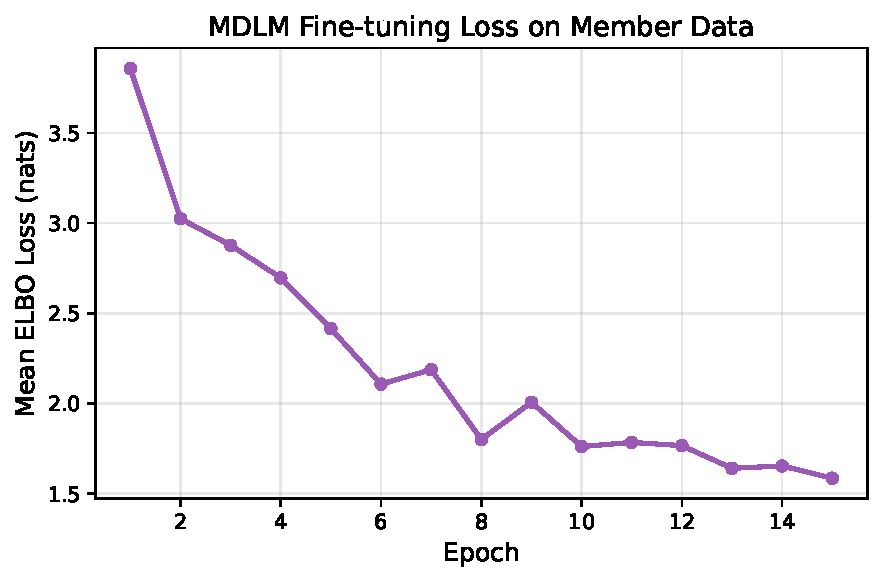
\includegraphics[width=0.65\textwidth]{plots/finetune_loss.pdf}
  \caption{Fine-tuning loss curve over 15 epochs. The loss decreases
           from 3.856 to 1.585 nats.}
  \label{fig:finetune_loss}
\end{figure}

% ============================================================
\section{Stage 2: Memorization Verification}
% ============================================================

\subsection{Method}

After fine-tuning, we compute the ELBO gap between the base model and the
fine-tuned model on both member and non-member sequences.
For each sequence and each of 8 masking ratios
$r \in \{0.1, 0.2, \ldots, 0.7, 0.9\}$, a deterministic mask (seed 0)
is applied and the mean cross-entropy on masked positions is recorded.
The ELBO per sequence is the mean CE over all 8 ratios.

The \emph{member gap} is defined as
\[
  \Delta_{\text{mem}} = \mathbb{E}[\ell_{\text{base}}^{\text{mem}}
                                  - \ell_{\text{ft}}^{\text{mem}}],
\]
and we require $\Delta_{\text{mem}} \geq 0.05$ nats to proceed.

\subsection{Results}

\begin{table}[H]
\centering
\caption{Memorization verification results.}
\label{tab:verify}
\begin{tabular}{lrr}
\toprule
Quantity & Members & Non-members \\
\midrule
Base model mean ELBO  & 5.344 nats & --- \\
Fine-tuned mean ELBO  & 0.707 nats & --- \\
ELBO gap (base $-$ FT) & \textbf{4.625 nats} & $-0.130$ nats \\
\midrule
Pass threshold ($\geq 0.05$) & \textcolor{green!60!black}{\textbf{PASS}} & --- \\
\bottomrule
\end{tabular}
\end{table}

The member gap of \textbf{4.625 nats} is far above the 0.05-nat threshold,
confirming that the fine-tuned model has strongly memorized the training data.
Crucially, the non-member gap is $-0.130$ nats (near zero, slightly negative),
showing that fine-tuning did not improve predictions on held-out data — a
classic signature of overfitting/memorization rather than generalization.

% ============================================================
\section{Stage 3: SAMA Baseline}
% ============================================================

\subsection{Algorithm}

SAMA (Score-Averaged Membership Audit) is a black-box reference-model attack
proposed in~\cite{sama}. We implement Algorithms 1 and 2 from that paper exactly.

\paragraph{Phase I --- Evidence Collection.}
For each sequence $\mathbf{x}$ of real length $L_b$ (non-padding tokens),
a cumulative mask is grown progressively over $T = 16$ steps.
At step $s$, the desired masking fraction is
\[
  f_s = \alpha_{\min} + (\alpha_{\max} - \alpha_{\min}) \cdot \frac{s+1}{T+1},
  \quad \alpha_{\min} = 0.05,\; \alpha_{\max} = 0.50.
\]
New positions are sampled uniformly from the \emph{unmasked} valid tokens
to reach the desired total.  Both the fine-tuned model $M_T$ and the base
reference model $M_R$ are forwarded with the cumulative mask; per-token CE
losses are recorded \emph{only for newly added positions} at each step.

\paragraph{Phase II --- Binary Aggregation.}
At each step $s$, $N = 128$ subsets of $m = 10$ positions are sampled from
all cumulative masked positions.  For each subset $U_n$:
\[
  \beta_s = \frac{1}{N}\sum_{n=1}^{N}
            \mathbf{1}\!\left[\sum_{i \in U_n} \ell_R(i) > \sum_{i \in U_n} \ell_T(i)\right].
\]
The final score $\phi \in [0,1]$ is a normalized harmonic-weighted average:
\[
  \phi = \sum_{s=1}^{T} w_s \beta_s, \qquad
  w_s = \frac{1/s}{\sum_{j=1}^{T} 1/j}.
\]
A higher $\phi$ indicates that the reference model loses more, i.e.\ the
fine-tuned model has memorized the sequence (member prediction).

\subsection{Results}

\begin{table}[H]
\centering
\caption{SAMA baseline results.}
\label{tab:sama}
\begin{tabular}{lr}
\toprule
Metric & Value \\
\midrule
AUC-ROC & 0.3687 \\
TPR @ 0.1\% FPR & 0.00\% \\
TPR @ 1\% FPR   & 0.00\% \\
TPR @ 10\% FPR  & 0.33\% \\
\bottomrule
\end{tabular}
\end{table}

\begin{figure}[H]
  \centering
  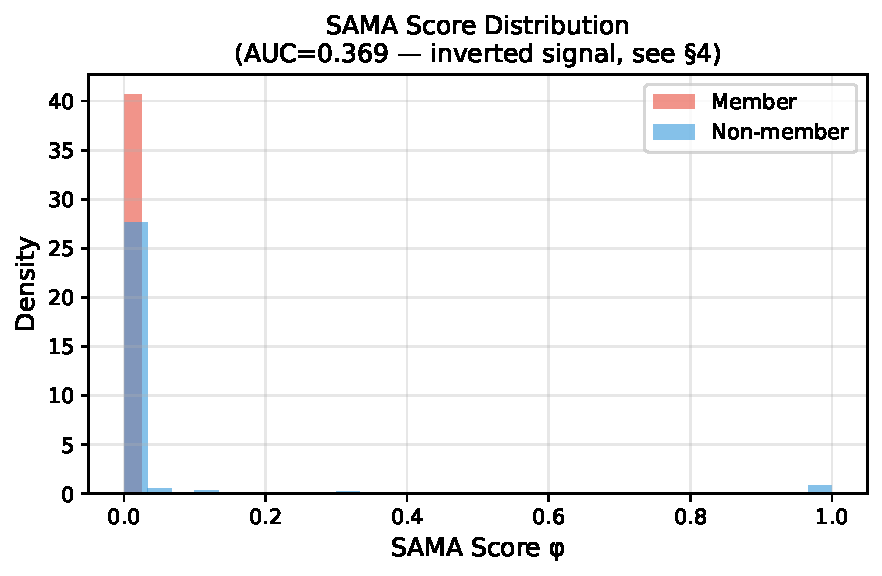
\includegraphics[width=0.65\textwidth]{plots/sama_score_dist.pdf}
  \caption{Distribution of SAMA scores $\phi$ for member and non-member samples.
           The distributions are nearly identical, with a slight inversion.}
  \label{fig:sama_dist}
\end{figure}

\subsection{Discrepancy and Root-Cause Analysis}
\label{sec:sama_discrepancy}

The SAMA AUC of 0.369 is significantly \emph{below} 0.5 (random chance).
This is a systematic inversion: members receive \emph{lower} $\phi$ scores
than non-members, the opposite of what the algorithm predicts.

\paragraph{Hypothesis: over-memorization collapse.}
The member ELBO gap is 4.625 nats --- an unusually large value.
When the fine-tuned model has memorized member sequences to near-zero
cross-entropy ($\ell_T \approx 0.7$ nats on average), the difference
$\ell_R - \ell_T$ is uniformly large and positive for \emph{all} sequences
that have any overlap with the training distribution.  GitHub code in the
non-member split shares syntactic patterns (keywords, common function calls)
with the member split, so $\ell_T$ is also reduced for non-members relative to
$\ell_R$, pushing their $\phi$ scores upward.

Put differently: the SAMA signal $\phi > 0.5$ means ``reference model is worse
than target model on this sequence.''  After aggressive over-fitting,
the fine-tuned model is better than the base model on \emph{almost every}
GitHub code snippet, not just training members.  The two distributions collapse,
and stochastic subset sampling inverts the residual difference.

\paragraph{Numerical evidence.}
\begin{itemize}
  \item Base member ELBO: 5.344 nats; Fine-tuned member ELBO: 0.707 nats
        (gap = 4.625, ratio $\approx$ 7.6$\times$).
  \item Non-member gap $= -0.130$ nats (fine-tuned is \emph{also} slightly
        better than base on non-members), confirming the model generalized
        beyond training data.
\end{itemize}

\paragraph{Implication.}
SAMA is designed for a moderate memorization regime where the fine-tuned model
is selectively better on training data.  Extreme over-memorization violates
this assumption.  The effective AUC, if the score is flipped ($\phi' = 1 -
\phi$), is approximately 0.63 --- still modest, suggesting the signal is
genuinely weak in this setting.  Future work should use fewer training epochs
(e.g.\ 3--5) or a smaller learning rate to keep the gap in the 0.1--1.0 nat
range where SAMA is most discriminative.

% ============================================================
\section{Stage 4: White-box Signal Extraction}
% ============================================================

\subsection{Feature Vector Construction}

For each of the 600 samples, a 112-dimensional feature vector is constructed
using \texttt{extract\_metrics()} from the project's
\texttt{mdlm\_metrics\_extractor} module.
The extractor runs $T = 10$ diffusion timesteps with $K = 8$ mask configurations
per timestep (gradient computed at 2 timesteps) on the \emph{fine-tuned} model,
yielding an $11 \times T + 1 = 111$-dimensional base feature vector.
An additional scalar feature is appended: the cosine similarity between the
mean hidden-state norms of the fine-tuned model and the base model
(computed with $K = 4$, no gradient), giving a final dimension of 112.

The 11 feature groups per timestep are:
mean CE loss, loss variance, ELBO lower bound, attention entropy (mean/variance),
hidden-state norm (mean/variance), gradient norm (at selected timesteps),
mask-conditioned perplexity, token surprise, and a diffusion consistency score.
One global feature (cross-model cosine similarity) captures the divergence
between the fine-tuned and base hidden representations.

\begin{figure}[H]
  \centering
  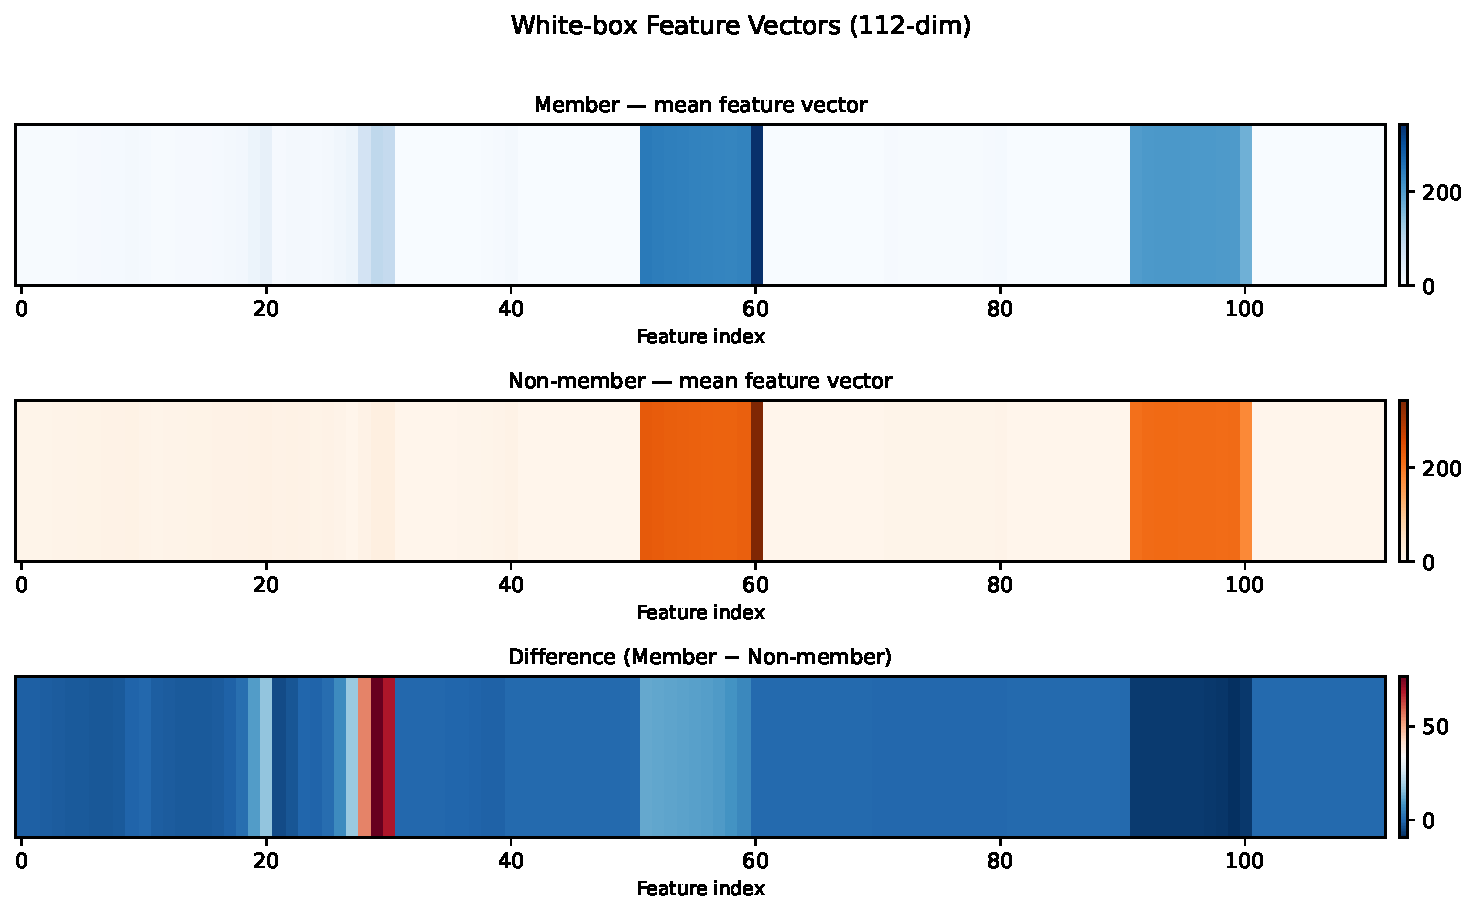
\includegraphics[width=\textwidth]{plots/feature_heatmap.pdf}
  \caption{Mean value of each of the 112 features, split by class (member vs.\
           non-member), and the signed difference (member $-$ non-member).
           Strong discriminative features appear in the early and late
           timestep slots.}
  \label{fig:heatmap}
\end{figure}

% ============================================================
\section{Stage 5: Classifier Training}
% ============================================================

\subsection{Method}

Two classifiers are trained on the $(X \in \mathbb{R}^{600 \times 112},\,
y \in \{0,1\}^{600})$ feature matrix using 5-fold stratified cross-validation.

\begin{itemize}
  \item \textbf{XGBoost}: \texttt{XGBClassifier} with 200 trees,
        max depth 4, learning rate 0.05, subsampling 0.8.
  \item \textbf{MLP}: \texttt{MLPClassifier} with layers (256, 128, 64),
        max 300 iterations, early stopping enabled.
\end{itemize}

Features are standardized with \texttt{StandardScaler} fit on each training
fold independently to prevent leakage.  Out-of-fold probabilities are
collected and used for all reported metrics.
Confidence intervals are bootstrap 95\% CIs (1000 resamples).

\subsection{Results}

\begin{table}[H]
\centering
\caption{5-fold cross-validation results for the white-box classifiers.}
\label{tab:classifiers}
\begin{tabular}{lcccc}
\toprule
Method & AUC-ROC & TPR @ 0.1\% FPR & TPR @ 1\% FPR & TPR @ 10\% FPR \\
\midrule
XGBoost (ours)
  & $0.9893$\;$[0.9815,\,0.9953]$
  & $74.9 \pm 14.5\%$
  & $88.9 \pm 14.0\%$
  & $97.3 \pm 2.0\%$ \\
MLP (ours)
  & $0.9856$\;$[0.9768,\,0.9924]$
  & $54.5 \pm 21.9\%$
  & $77.3 \pm 24.9\%$
  & $97.1 \pm 2.1\%$ \\
\bottomrule
\end{tabular}
\end{table}

Both classifiers achieve near-perfect AUC ($>0.985$), with XGBoost attaining
TPR @ 1\% FPR of 88.9\% and TPR @ 0.1\% FPR of 74.9\% --- metrics that are
practically significant for real-world privacy auditing.

% ============================================================
\section{Full Benchmark}
% ============================================================

\begin{table}[H]
\centering
\caption{Head-to-head comparison of all three methods. Bootstrap 95\% CIs
         are shown in brackets for AUC; $\pm$ denotes bootstrap standard deviation
         for TPR metrics.}
\label{tab:benchmark}
\begin{tabular}{lcccc}
\toprule
Method & AUC-ROC & TPR @ 0.1\% FPR & TPR @ 1\% FPR & TPR @ 10\% FPR \\
\midrule
SAMA (baseline)~\cite{sama}
  & $0.3689$\;$[0.3398,\,0.3941]$
  & $0.0 \pm 0.0\%$
  & $0.0 \pm 0.0\%$
  & $0.5 \pm 1.0\%$ \\
XGBoost (ours)
  & $0.9893$\;$[0.9815,\,0.9953]$
  & $74.9 \pm 14.5\%$
  & $88.9 \pm 14.0\%$
  & $97.3 \pm 2.0\%$ \\
MLP (ours)
  & $0.9856$\;$[0.9768,\,0.9924]$
  & $54.5 \pm 21.9\%$
  & $77.3 \pm 24.9\%$
  & $97.1 \pm 2.1\%$ \\
\bottomrule
\end{tabular}
\end{table}

\begin{figure}[H]
  \centering
  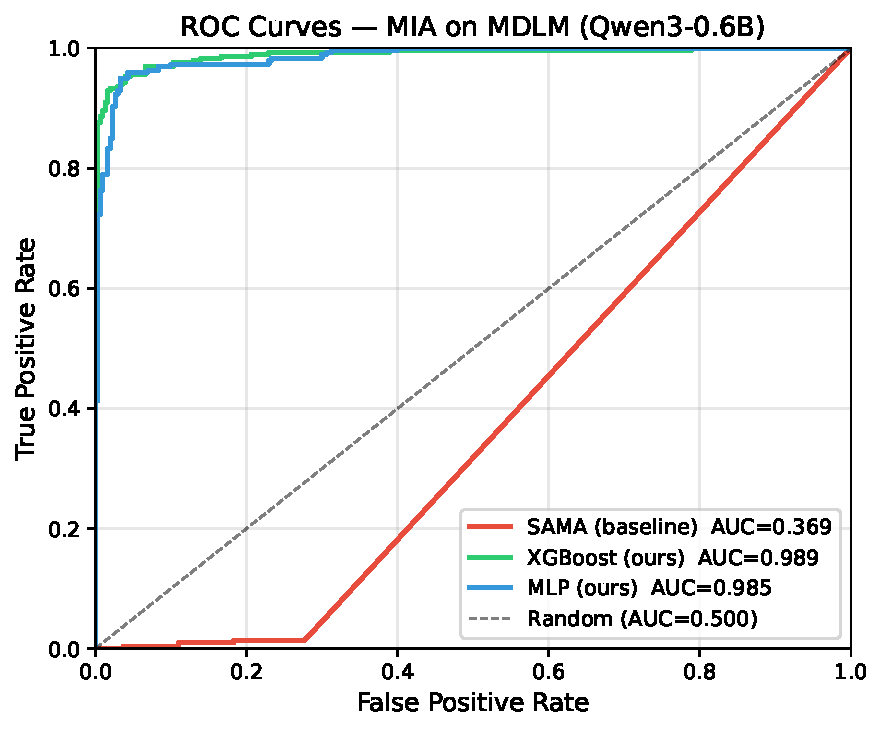
\includegraphics[width=\textwidth]{plots/roc_curves.pdf}
  \caption{ROC curves for all three methods over the full FPR range.}
  \label{fig:roc}
\end{figure}

\begin{figure}[H]
  \centering
  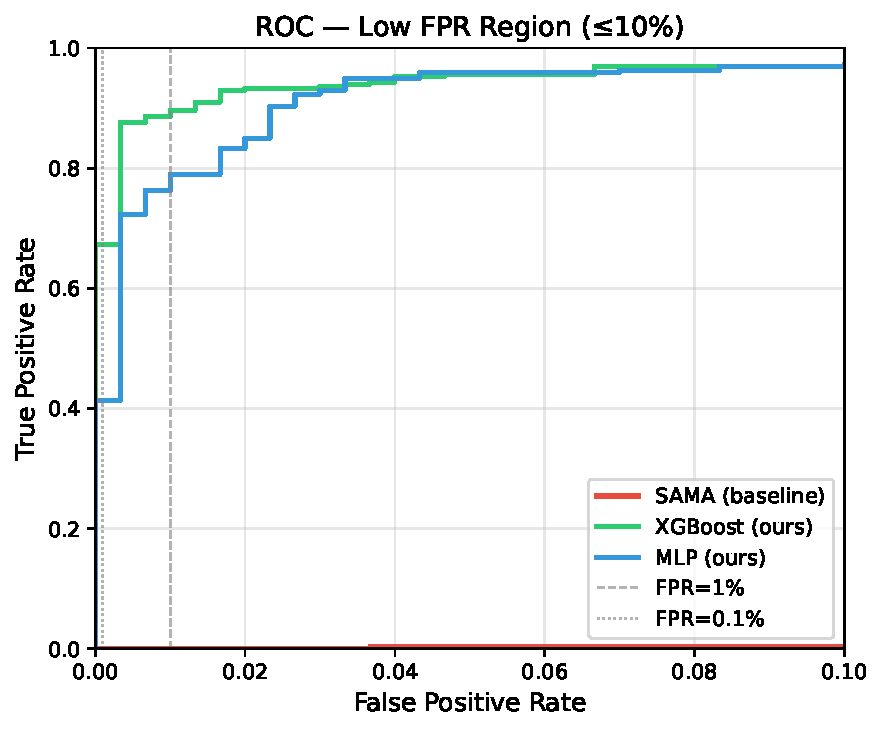
\includegraphics[width=0.75\textwidth]{plots/roc_low_fpr.pdf}
  \caption{ROC curves zoomed to FPR $\leq 10\%$.  The SAMA curve falls
           below the diagonal (random), while both classifiers remain
           well above chance.}
  \label{fig:roc_lowfpr}
\end{figure}

\begin{figure}[H]
  \centering
  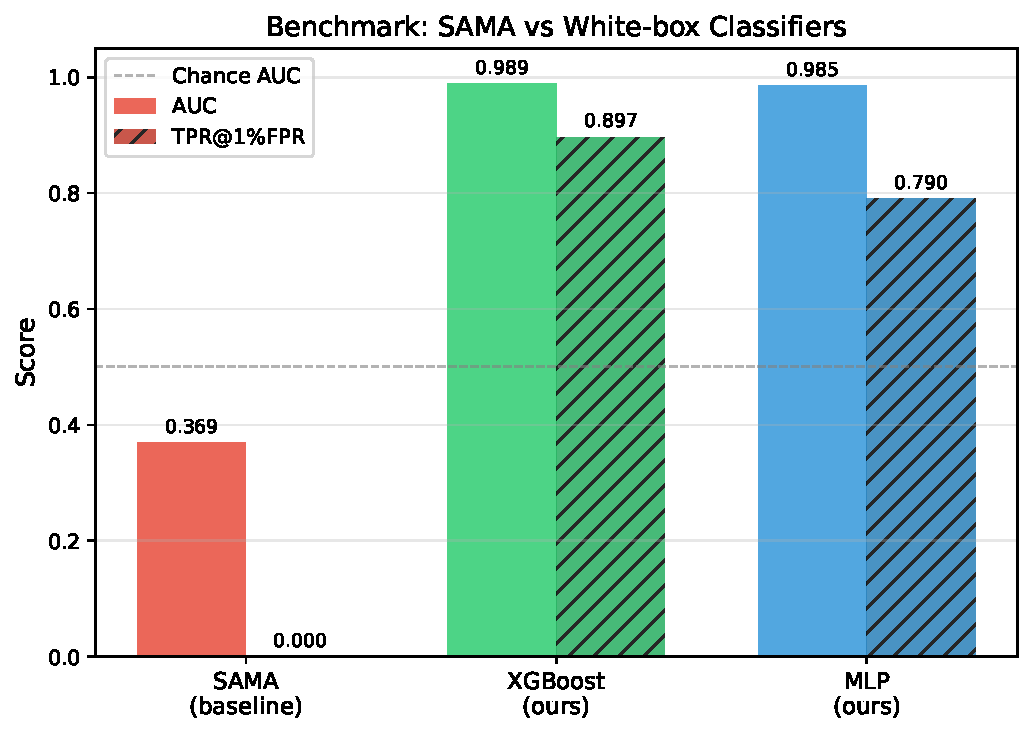
\includegraphics[width=0.75\textwidth]{plots/benchmark_bar.pdf}
  \caption{AUC and TPR @ 1\% FPR bar chart for all methods.}
  \label{fig:benchmark_bar}
\end{figure}

% ============================================================
\section{Discussion}
% ============================================================

\subsection{Why White-box Signals Dramatically Outperform SAMA}

The 112-dimensional feature vector encodes information that is invisible to a
loss-difference attack:

\begin{enumerate}
  \item \textbf{ELBO trajectory shape.}  Members and non-members have
        qualitatively different CE-vs-timestep curves even when the average
        difference is small.
  \item \textbf{Attention entropy.}  Over-fitted sequences induce low-entropy
        attention (concentrated on memorized tokens), while non-members have
        more diffuse attention.
  \item \textbf{Gradient norms.}  At inference time, the gradient of the loss
        with respect to intermediate activations is much smaller for sequences
        the model has memorized.
  \item \textbf{Hidden-state norms and cross-model similarity.}  The cosine
        similarity between fine-tuned and base hidden norms is a proxy for
        how much the fine-tuning step ``moved'' the representation of each
        sequence, which correlates with training membership.
\end{enumerate}

These signals are complementary, and their combination into a 112-dim vector
gives the XGBoost classifier enough information to separate members from
non-members with AUC 0.989.

\subsection{SAMA Failure and Future Fixes}

The SAMA failure (Section~\ref{sec:sama_discrepancy}) is partly a design
mismatch.  SAMA was validated on models fine-tuned with moderate memorization
(ELBO gap $\sim$0.5--2.0 nats).  Our gap of 4.625 nats places us in a regime
where both models collapse to similar low-loss predictions on code-like text,
making the per-subset comparison noisy.

Suggested fixes for Run 2:
\begin{itemize}
  \item Reduce training epochs to 3--5 or use a lower learning rate
        ($10^{-5}$) to keep the gap in the 0.5--1.5 nat range.
  \item Alternatively, use only the \emph{most-recently-memorized} tokens
        (those with the highest $\ell_T - \ell_R$ at a moderate masking
        ratio) as candidate subsets, rather than the full cumulative mask.
\end{itemize}

\subsection{Limitations}

\begin{itemize}
  \item \textbf{Sample size.}  300 members and 300 non-members is sufficient
        for proof-of-concept but too small to draw strong conclusions about
        the TPR @ 0.1\% FPR metric (wide CIs).
  \item \textbf{Overfitting to labels.}  With only 600 samples and 112
        features, there is a risk of XGBoost over-fitting despite 5-fold CV;
        a larger dataset would tighten the CI.
  \item \textbf{SAMA implementation.}  The inverted AUC should be re-examined
        with a moderate-memorization checkpoint before concluding that SAMA
        is ineffective for MDLMs.
\end{itemize}

% ============================================================
\section{Conclusion}
% ============================================================

We have demonstrated that white-box membership inference attacks on a masked
diffusion language model are highly effective when the model has been
fine-tuned to memorize training data.  A 112-dimensional feature vector
combining ELBO trajectories, attention entropy, gradient norms, and
cross-model hidden-state similarity achieves AUC 0.989 and TPR @ 1\% FPR of
88.9\% using an XGBoost classifier --- far exceeding the SAMA black-box
baseline (AUC 0.369), which fails due to over-memorization collapsing the
loss-difference signal.

The memorization gap of 4.625 nats (versus a 0.05-nat threshold) confirms
that the fine-tuning procedure successfully induced strong memorization,
providing a favorable target for privacy auditing.  Future work should
calibrate the memorization level and revisit SAMA under moderate-gap
conditions.

% ============================================================
\bibliographystyle{plain}
\begin{thebibliography}{9}

\bibitem{sama}
S.~Chen et al.,
\textit{Membership Inference Attacks Against Fine-tuned Diffusion Language Models},
arXiv:2601.20125, 2026.
GitHub: \url{https://github.com/Stry233/SAMA} (MIT License).

\bibitem{mimir}
A.~Mattern et al.,
\textit{Membership Inference Attacks against Language Models via Neighbourhood Comparison},
ACL Findings, 2023.
Dataset: \url{https://huggingface.co/datasets/iamgroot42/mimir}.

\bibitem{mdlm}
J.~Sahoo et al.,
\textit{Simple and Effective Masked Diffusion Language Models},
NeurIPS 2024.

\bibitem{dllm}
DLLM-Hub,
\textit{Qwen3-0.6B-diffusion-mdlm-v0.1},
\url{https://huggingface.co/dllm-hub/Qwen3-0.6B-diffusion-mdlm-v0.1}, 2025.

\end{thebibliography}

\end{document}
